\documentclass{article}

% NeurIPS 2026 style — default = anonymous double-blind submission
\usepackage{neurips_2026}

% Standard NeurIPS packages
\usepackage[utf8]{inputenc}
\usepackage[T1]{fontenc}
\usepackage{hyperref}
\usepackage{url}
\usepackage{booktabs}
\usepackage{amsfonts}
\usepackage{nicefrac}
\usepackage{microtype}
\usepackage{xcolor}
\usepackage{graphicx}
\usepackage{multirow}

% Colored prompt boxes
\usepackage[most]{tcolorbox}

\definecolor{PromptBlue}{HTML}{F3F8FF}
\definecolor{PromptFrame}{HTML}{2F5D9B}
\definecolor{PromptTitle}{HTML}{E7F0FF}

\newtcolorbox[auto counter]{promptbox}[2][]{
  enhanced,
  breakable,
  colback=PromptBlue,
  colframe=PromptFrame,
  coltitle=black,
  colbacktitle=PromptTitle,
  title={Prompt~\thetcbcounter: #2},
  fonttitle=\bfseries\small,
  fontupper=\small,
  boxrule=0.5pt,
  arc=1.2mm,
  left=1.2mm,
  right=1.2mm,
  top=1mm,
  bottom=1mm,
  toptitle=0.7mm,
  bottomtitle=0.7mm,
  attach boxed title to top left={xshift=1.5mm,yshift=-1.2mm},
  boxed title style={
    boxrule=0pt,
    arc=1mm,
    left=1mm,
    right=1mm,
    top=0.4mm,
    bottom=0.4mm
  },
  #1
}

\title{Survey Simulation Should Be Treated as Population Bridging, Not Respondent Simulation}

% Anonymous submission — do not include author names or affiliations
\author{
  Anonymous Author(s)
}

\begin{document}

\maketitle

\begin{abstract}
Social media offers a promising but biased source of population signal for LLM-based survey simulation. We frame this task as a population-bridging problem: real surveys measure a target population, LLMs reflect an implicit model population, and domain-specific social media provides an observed mediator between them. Using 12,000 Weibo and Xiaohongshu posts in Chinese consumer health and a benchmark survey with 138,000 responses, we compare a $2\times2$ design space that separates the response estimator (semantic mapping versus LLM simulation) from the population (unit---post-level versus population-structured inference). Across both estimators, recovering latent social-media groups before aggregation improves alignment with real survey distributions, reducing mean JS divergence from 0.0295 to 0.0269 for semantic mapping and from 0.0328 to 0.0275 for LLM simulation. The gains remain stable across alternative cluster-weighting schemes and are strongest when a moderate number of clusters is used. These results suggest that the key challenge in survey simulation is not only generating plausible answers, but choosing the right population unit for inference. Social media is most useful not as a flat pool of posts, but as a structured mediator population through which LLMs and embedding methods can better approximate real survey distributions.
\end{abstract}

\section{Introduction}

\begin{figure}[htb!]
\centering
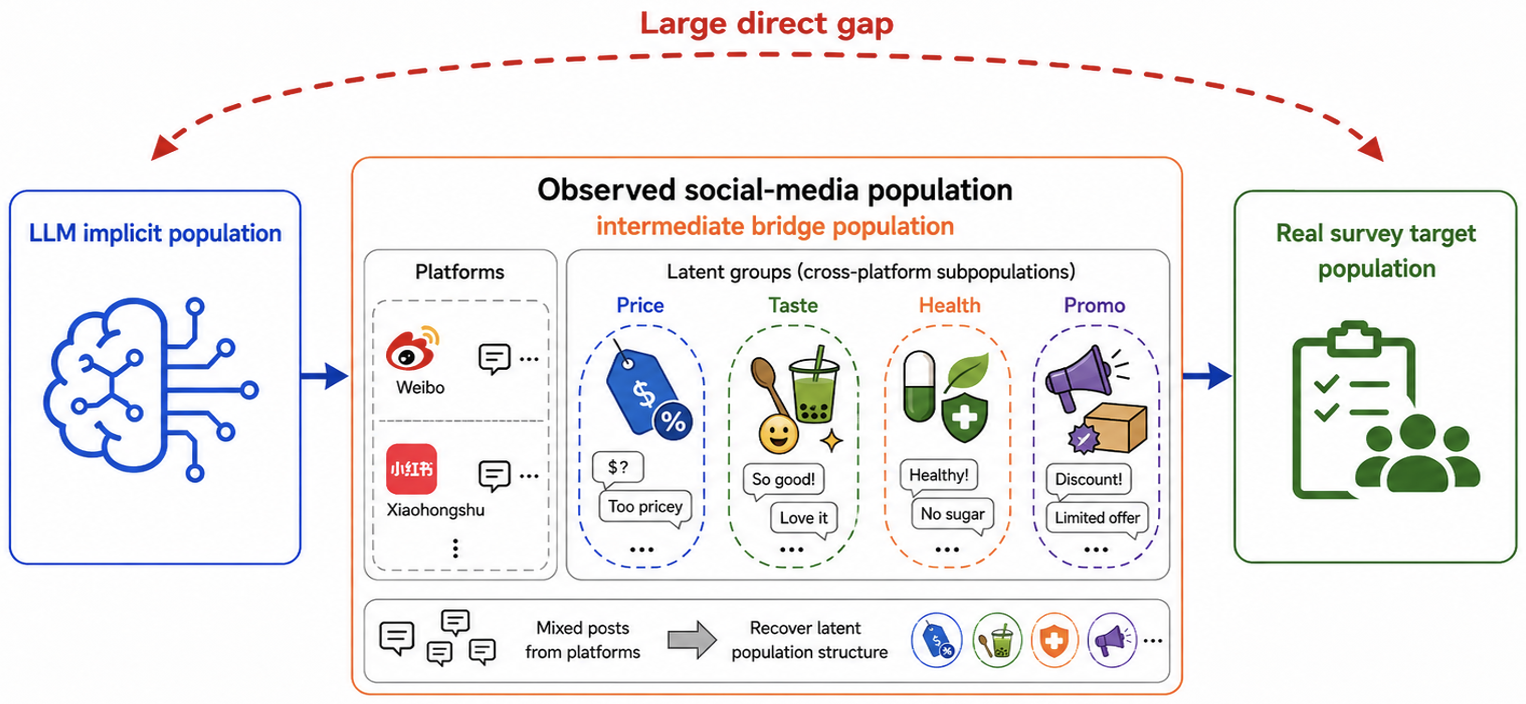
\includegraphics[width=0.9\linewidth]{bridge.png}
\caption{Population bridging through an observed social-media population. Social media is treated as an intermediate population that mediates between the LLM's implicit population and the real survey population.}
\label{bridge}
\end{figure}

Surveys provide structured measurements of population-level opinions,
preferences, and behaviors, but their high cost and slow cadence limit
real-time applicability.
This has motivated growing interest in using large language models
(LLMs) to approximate survey answer distributions.

Existing work approaches this problem in different ways.
One line prompts LLMs to generate survey responses directly,
often conditioning on demographic profiles, personas, or respondent
descriptions~\cite{aher2023using, argyle2023silicon, santurkar2023whose,
yang2024specializing}.
Another line avoids direct response generation by mapping free-form text
to survey scales through embedding similarity~\cite{maier2026llms}.
These two lines differ in how they estimate a response distribution:
one relies on LLM simulation, while the other relies on semantic mapping.

A separate design choice concerns the unit over which responses are
aggregated.
Many methods estimate responses for individual simulated respondents or
individual text inputs and then average them.
Other work introduces population structure through demographic strata,
population alignment, or persona mixtures~\cite{wang2024mixture,
hwang2023aligning}.
These approaches suggest that the aggregation unit matters:
a survey distribution is not only a collection of independent responses,
but also a population-level object whose estimate depends on how the
underlying population is represented.

This creates a population mismatch that is often implicit in
LLM-based survey simulation (Fig.\ref{bridge}).
A real survey measures a target population.
An LLM draws on an implicit population induced by its training corpus,
world knowledge, and alignment behavior.
If the model is used as the only source of population signal, the
predicted distribution may reflect the LLM's implicit population rather
than the real survey population.
External population evidence can help, but it introduces its own design
questions:
given such evidence, how should it be converted into survey answer
distributions, and at what population unit should the resulting estimates
be aggregated?

Observed online data is one possible source of such evidence.
Prior work on social data as a survey proxy shows that online platforms
can contain useful population signal~\cite{wang2015forecasting,
cerina2024ai}.
At the same time, online populations are non-representative, noisy, and
demographically unstable~\cite{diaz2016online}, and demographic
reweighting can fail when coverage is sparse or missing~\cite{sen2017total}.
Thus, observed domain data is neither an unbiased survey sample nor a
pure model prior.
It occupies an intermediate position: it contains empirical evidence
from the target domain, but its relationship to the real survey
population must be modeled.

We therefore study the following question:
\textit{given an observed domain population, which combination of
response estimator and population unit best approximates a real survey
distribution?}
To answer this question, we organize the design space as a
$2\times2$ comparison (Fig.\ref{2by2}).
One axis is the response estimator:
semantic mapping versus LLM simulation.
The other axis is the population unit:
post-level inference versus population-structured inference.
This framework lets us separate two effects that are often conflated:
whether performance comes from the estimator used to map text to survey
answers, or from the way the observed population is represented and
aggregated.

In our empirical setting, the observed population is a domain-specific
social-media corpus from Weibo and Xiaohongshu.
These platforms contain large volumes of user-generated content that
reflect public attitudes and domain-specific experiences at
scale~\cite{wang2015forecasting, cerina2024ai}.
In the Chinese consumer health domain, posts capture survey-relevant
expressions such as symptoms, product use, seasonal contexts, and
treatment experiences.
We evaluate the four cells of the $2\times2$ framework against a real
Chinese consumer health survey benchmark.

Our results show that the key design choice is the population unit.
Across both response estimators, using the observed corpus through
recovered population structure improves over treating it as a flat
collection of posts.
This suggests that, in our setting, observed social media is most useful
not simply as more text for an LLM or an embedding model,
but as a mediator population whose internal structure must be recovered
before aggregation.

Our contributions are threefold.
\textbf{(i)} We frame LLM-based survey simulation as a population
mismatch problem involving the real survey population, the LLM's
implicit population, and an observed domain population.
\textbf{(ii)} We introduce a $2\times2$ diagnostic framework that
separates response-estimator choice from population-unit choice,
comparing semantic mapping and LLM simulation under post-level and
population-structured inference.
\textbf{(iii)} We instantiate this framework in Chinese consumer health
survey simulation using approximately 12,000 Weibo and Xiaohongshu posts
evaluated against a 138,000-response benchmark survey, and find that
recovering latent population structure before aggregation consistently
reduces divergence from the real survey distribution.

\section{Related Work}

\subsection{LLM-Based Survey Simulation}

A growing body of work studies whether large language models can simulate
survey respondents or reproduce population-level opinion distributions.
Early work on ``silicon samples'' and simulated human subjects prompts LLMs
to answer as individuals with specified demographic profiles, personas, or
experimental contexts~\cite{aher2023using,argyle2023silicon}.
Subsequent studies examine how closely model responses match human opinion
data, and how model outputs vary across demographic conditioning, political
attitudes, and social groups~\cite{santurkar2023whose}.
More recent work further trains or adapts LLMs to predict survey response
distributions across countries and populations~\cite{yang2024specializing}.
Together, these studies demonstrate that LLMs can reproduce some aggregate
patterns in survey data and can serve as useful tools for large-scale
response simulation.

However, direct LLM simulation raises a population-representation problem.
When an LLM is asked to answer a survey, the response distribution is shaped
not only by the prompt, but also by the model's training corpus, world
knowledge, and alignment behavior.
Demographic or persona conditioning can steer the model toward a desired
respondent profile, but the resulting distribution still depends heavily on
the model's implicit prior over what such respondents are like.
Thus, even when outputs appear plausible, it is unclear whether the model is
representing the target survey population or the model's internalized
approximation of that population.
Our work makes this mismatch explicit and studies how an observed domain
population can be used as an external mediator.

A complementary line avoids direct survey response generation.
Semantic Similarity Rating (SSR) maps free-form text to survey answer options
through embedding similarity~\cite{maier2026llms}.
Rather than asking a model to generate an answer, SSR embeds both the input
text and answer-option anchors in a shared semantic space, then derives a
response distribution from similarity scores.
This separates text representation from direct answer generation and can
provide stable distributional estimates.
In our framework, SSR-style semantic mapping and direct LLM simulation are
treated as two alternative response estimators.
This lets us ask whether performance differences arise from the estimator
itself or from the population unit over which estimates are aggregated.

\subsection{Population Alignment, Personas, and Demographic Structure}

Because surveys measure population-level quantities, several recent methods
explicitly model population structure.
Persona-based simulation constructs synthetic respondents with demographic,
behavioral, or attitudinal attributes, then aggregates their simulated
responses.
Mixture-of-personas approaches learn or sample weighted persona profiles so
that simulated outputs better match target populations~\cite{wang2024mixture}.
Other methods align generated populations with demographic targets using
importance sampling, optimal transport, or related reweighting procedures
~\cite{hwang2023aligning}.
These methods recognize that the aggregation unit matters:
the final survey distribution depends not only on how each response is
generated, but also on which respondents or groups are represented and how
they are weighted.

This line of work is closely related to our population-unit dimension, but
differs in how population structure is obtained.
Existing population-alignment methods often assume that the relevant
structure is known in advance, for example through demographic categories,
census targets, or predefined persona schemas.
This is appropriate when reliable metadata is available and when the
survey-relevant dimensions are well captured by those variables.
In many social-media settings, however, demographic information is missing,
noisy, or too sparse to support reliable post-stratification.
Moreover, survey-relevant variation may be topical or contextual rather than
strictly demographic: product-use scenarios, symptom communities, seasonal
contexts, or promotional audiences may all influence responses.
Our work therefore recovers latent groups empirically from the observed
corpus itself and uses those groups as population units for aggregation.

\subsection{Social Media as a Survey Proxy}

Social media has long been studied as a potential proxy for measuring public
opinion and population behavior.
Pre-LLM work shows that non-representative online data can approximate
survey or election outcomes when combined with appropriate population
correction.
For example, multilevel regression with post-stratification can correct
substantial sampling bias when demographic information is available
~\cite{wang2015forecasting}.
At the same time, social-media platforms have been characterized as
imperfect continuous panels: they provide large-scale, frequently updated
signals, but exhibit strong demographic skew, platform effects, and temporal
instability~\cite{diaz2016online}.
Other work shows that demographic reweighting can fail when social-media
coverage is sparse or when important groups are missing from the observed
sample~\cite{sen2017total}.

Recent LLM-era work revisits social media as a source of opinion evidence.
LLMs can extract opinions, topics, or issue positions from noisy text and
combine them with population models for downstream estimation
~\cite{cerina2024ai}.
Agentic systems further use LLMs to gather and summarize social-media
opinions at scale~\cite{surveypilot2024}.
These approaches highlight the value of social media as observed domain
evidence, but they often treat the corpus as a flat collection of posts or
rely on external demographic correction to make it population-relevant.
This leaves open the question of how to use social data when demographic
metadata is unavailable and the corpus itself is heterogeneous.

Our work treats social media as an observed mediator population rather than
as either a representative survey sample or a flat text corpus.
The key assumption is not that social media is unbiased, but that its
internal structure contains survey-relevant population signal.
By recovering latent topic groups and aggregating through those groups, we
use social media to mediate between the LLM's implicit population and the
real survey population.
This differs from classical post-stratification, which relies on observed
demographic cells, and from direct LLM simulation, which relies primarily on
the model's internal prior.
Representative posts illustrating the platform-level discourse patterns in our corpus are shown in Table~\ref{tab:sm_examples} in Appendix~\ref{app:tables}.

\begin{table}[htb!]
\centering
\small
\begin{tabular}{p{0.08\textwidth}p{0.39\textwidth}p{0.45\textwidth}}
\toprule
Question ID & Survey question & Option list \\
\midrule
\multicolumn{3}{l}{\textbf{Panel A: Product-experience-oriented questions used for distributional evaluation}} \\
\midrule
Q1 &
How do you think the price of \{Product Name\}? &
A: Very expensive; B: Somewhat expensive; C: Reasonable; D: Cheap \\

Q2 &
In what season would you be likely to buy \{Product Name\}? &
A: Spring; B: Summer; C: Autumn; D: Winter; E: No seasonal preference \\

Q3 &
Which attribute matters when you buy \{Product Name\}? &
A: Effectiveness; B: Safety; C: Brand reputation; D: Price; F: Others \\

% \multicolumn{3}{c}{\ldots} \\
\midrule
\multicolumn{3}{l}{\textbf{Panel B: Demographic and background questions used for population characterization}} \\
\midrule
D1 &
Gender &
A: Male; B: Female; C: Other / prefer not to say \\

D2 &
Age group &
A: Under 18; B: 18--24; C: 25--34; D: 35--44; E: 45--54; F: 55 and above \\

D3 &
Province or city of residence &
Free-text response \\

% \multicolumn{3}{c}{\ldots} \\
\bottomrule
\end{tabular}
\caption{Representative questions from the benchmark survey. Product names are masked as \{Product Name\}. Panel A shows product-experience-oriented questions used for distributional evaluation, while Panel B shows demographic and background questions used to characterize the survey population and support population-level analysis. Some questions and options are omitted for brevity.}
\label{tab:questions}
\end{table}

\section{Problem Formulation and Design Space}
\label{sec:problem}

We study survey distribution estimation with three populations in mind:
the \emph{real survey population}, whose answer distribution is the target;
the \emph{LLM implicit population}, induced by the model's training data and alignment;
and an \emph{observed social-media population}, which is biased but domain-relevant.
Our goal is to use the observed social-media population as a mediator for estimating the real survey answer distribution.

For a survey question $q$ with answer options $\mathcal{Y}=\{1,\ldots,K\}$,
let $p^{\star}(y \mid q)$ denote the real survey distribution.
Given a social-media corpus $\mathcal{S}=\{s_i\}_{i=1}^{N}$,
we seek an estimator
\[
\hat{p}(y \mid q,\mathcal{S}) \approx p^{\star}(y \mid q).
\]

We organize the method space along two dimensions, shown in Figure~\ref{2by2}.
The first dimension is the \emph{response estimator}: how textual evidence is converted into a distribution over survey answers.
The second dimension is the \emph{population unit}: the unit over which response estimates are produced and aggregated.

\begin{figure}[htb!]
\centering
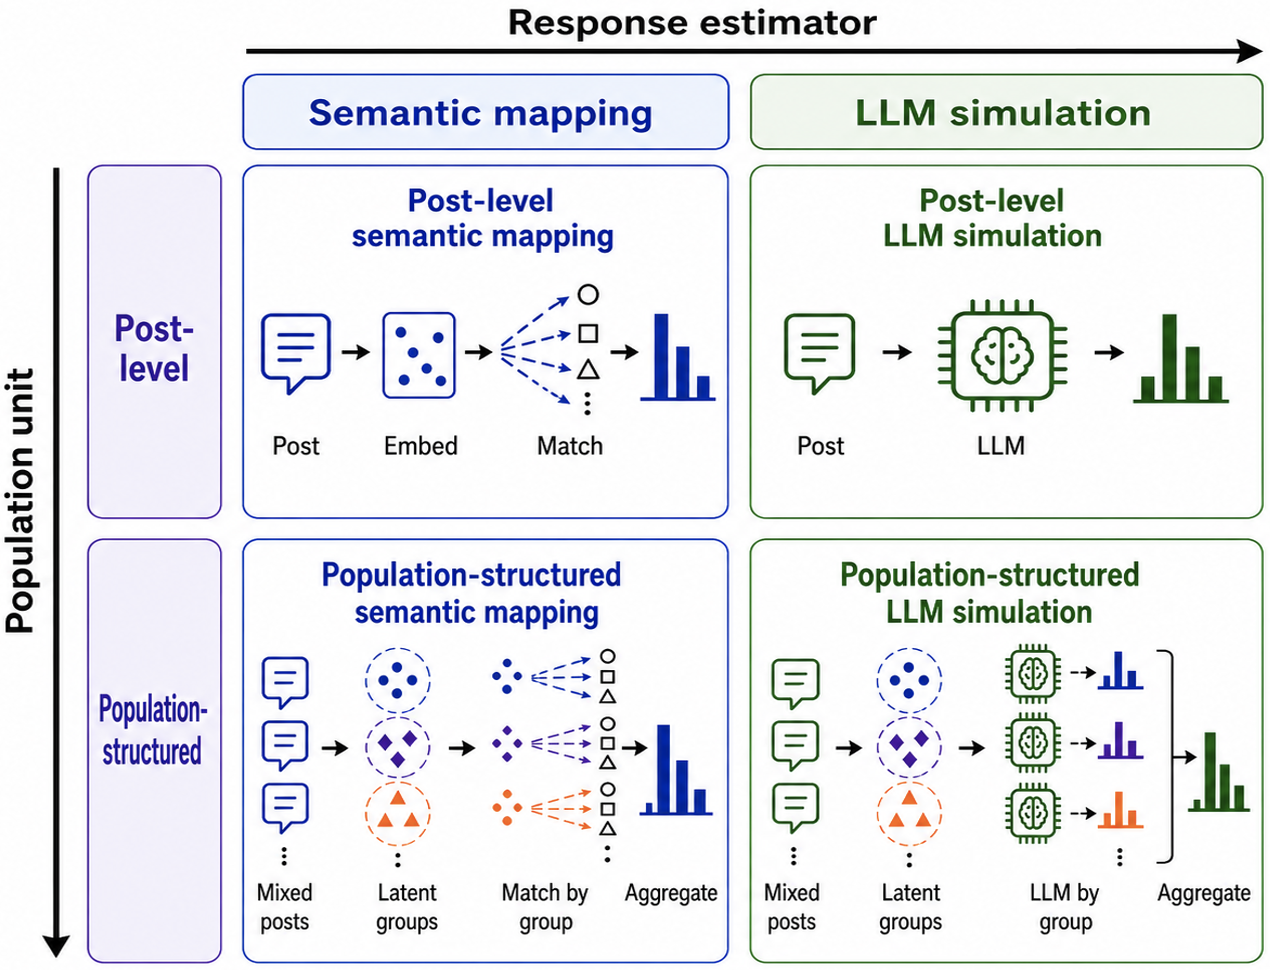
\includegraphics[width=0.65\linewidth]{2by2.png}
\caption{Two-by-two design space for social-media-based survey simulation.}
\label{2by2}
\end{figure}

\subsection{Response estimator}
A response estimator maps textual evidence $x$ to an answer distribution $f(y \mid q,x)$.
We consider two estimator families.
Semantic mapping estimates $f$ by comparing the semantic representation of $x$ with answer-option anchors.
LLM simulation estimates $f$ by prompting a language model to directly return a probability distribution over the answer options.
The detailed implementations are described in Sections~\ref{SSR_sec} and~\ref{LLM_prompt}.

\subsection{Population unit}
Under \emph{post-level inference}, each social-media post is treated as an independent unit:
\[
\hat{p}_{\mathrm{post}}(y \mid q,\mathcal{S})
=
\frac{1}{N}\sum_{i=1}^{N} f(y \mid q, s_i).
\]
This treats the observed corpus as a flat collection of posts.

Under \emph{population-structured inference}, the corpus is first organized into latent groups
$\mathcal{G}=\{G_1,\ldots,G_C\}$ with weights $\pi_c$ such that $\sum_{c=1}^{C}\pi_c=1$.
The final estimate aggregates group-level response distributions:
\[
\hat{p}_{\mathrm{struct}}(y \mid q,\mathcal{S})
=
\sum_{c=1}^{C} \pi_c \hat{p}_c(y \mid q,G_c).
\]
This treats social media as a structured mediator population rather than a flat sample.

Together, these two dimensions define four practices:
post-level semantic mapping, population-structured semantic mapping,
post-level LLM simulation, and population-structured LLM simulation.
This design lets us separate errors due to response estimation from errors due to population representation.

\section{Experiment}
\label{sec:experiment}

\subsection{Data}

\subsubsection{Social Media Data}
We collect approximately 12,000 posts from Weibo and Xiaohongshu in the Chinese consumer health / Traditional Chinese Medicine (TCM) domain.
The corpus focuses on discussions of over-the-counter TCM products,
including Huoxiang Zhengqi formulations, cough syrups, and cold medicines,
primarily from a major pharmaceutical brand.

\subsubsection{Survey Data}
We evaluate against a real-world Chinese consumer health survey with approximately 138,000 responses.
As summarized in Table~\ref{tab:questions}, the survey contains two types of questions:
product-experience-oriented questions and demographic/background questions.
Our main distributional evaluation uses the six human-authored, single-choice product-experience questions in Panel A.
The demographic and background questions in Panel B are used to characterize the survey population and support population-level analyses.
All reported evaluation results are based solely on real survey responses, so that the benchmark reflects genuine population distributions rather than model artifacts.

\subsubsection{Data Cleansing}

We clean the survey data by parsing each respondent's questionnaire record from a JSON-encoded content field and repairing common formatting artifacts when necessary. We restrict the data to the target survey and aggregate valid responses into option-level answer counts for each question.
Demographic and background questions are excluded from the main evaluation, and the final benchmark contains six product-experience questions with empirical answer distributions from real survey responses.

For the social-media corpus, we retain only Weibo and Xiaohongshu posts that mention the target product family.
We normalize text fields, remove hashtag wrappers, and filter out posts with confounding product meanings, recipes, parenting contexts, social mentions, bare reposts, or likely professional medical and health-care authors.
We then remove exact duplicates and near-duplicates using a 10-character sliding-window deduplication rule to reduce template reposts and minor variants.

After filtering and deduplication, the corpus contains 27,838 posts. Following HDBSCAN clustering as detailed in Section \ref{cluster_sec}, posts assigned to the noise label are removed, yielding the final 11,873-post corpus, organized into 66 recovered clusters.
This approximately 12K-post corpus is used as the observed social-media population throughout the experiments.

\subsection{Method}

\subsubsection{2-Dimensional Instantiation}

We instantiate the four cells of the design space in Section~\ref{sec:problem} using the cleaned social-media corpus and the six survey questions.
The two response estimators are implemented as semantic mapping and Qwen3-8B-based LLM simulation.
The two population units are individual posts and HDBSCAN-recovered social-media groups.

\begin{itemize}
    \item \textbf{Post-level semantic mapping.}
    Apply semantic mapping to each post and average the resulting distributions.

    \item \textbf{Population-structured semantic mapping.}
    Apply semantic mapping within each recovered group and aggregate group-level distributions using cluster weights.

    \item \textbf{Post-level LLM simulation.}
    Prompt Qwen3-8B with a single post and aggregate the resulting post-level distributions.

    \item \textbf{Population-structured LLM simulation.}
    Prompt Qwen3-8B with cluster-level context and aggregate the resulting group-level distributions using cluster weights.
\end{itemize}

The following sections describe the recovered groups, semantic mapping implementation, and LLM prompting strategy.

\subsubsection{Population Recovery by Clustering}
\label{cluster_sec}

We recover latent social-media groups by clustering post embeddings.
After product-name masking, text normalization, filtering, and deduplication, each post is encoded using bge-small-zh-v1.5 \cite{bge_small_zh_v15} for clustering.
We then reduce the post embeddings to a 50-dimensional space using UMAP and apply HDBSCAN to identify dense semantic groups while treating low-density posts as noise.
Posts assigned to HDBSCAN's noise label are removed, yielding 11,873 posts organized into 66 clusters.

Representative recovered clusters are shown in Table~\ref{tab:clusters} in Appendix~\ref{app:tables}. The clusters capture distinct survey-relevant contexts, including medical use, heatstroke prevention, and product perception. This illustrates why we treat the social-media corpus as a structured mediator population rather than a flat collection of posts: different groups encode different use cases, attitudes, and consumption contexts that may map differently to survey answer distributions.

Because the number of clusters used for response estimation can affect coverage and noise, we later conduct a Top-$K$ sensitivity analysis (see Section~\ref{sensitivity}), varying the number of retrieved clusters and showing that performance is strongest in a moderate range, around $K=10$--$15$.
Importantly, clustering uses only social-media text and does not use survey responses, so the population recovery step is unsupervised with respect to the evaluation target.

\subsubsection{Semantic Mapping}
\label{SSR_sec}
For each survey question, we first convert every answer option into a natural-language anchor sentence.
The anchors are generated by Qwen3-8B using a fixed prompt that asks the model to rewrite each option as a concrete sentence expressing the corresponding attitude or choice, while preserving the original option order.
This step produces one anchor sentence for each answer option.

Each anchor sentence and each social-media text unit are then encoded using bge-base-zh-v1.5 \cite{bge_base_zh_v15}.
Given a text unit $x$ and the anchor sentence $a_k$ for option $k$, we compute their cosine similarity:
\[
z_k(x) = \cos(e(x), e(a_k)).
\]
The similarity scores are converted into a probability mass function over answer options:
\[
f_{\mathrm{sem}}(y=k \mid q,x)
=
\frac{\exp(z_k(x)/\tau)}
{\sum_{j=1}^{K}\exp(z_j(x)/\tau)},
\]
where $\tau$ is a temperature parameter controlling the sharpness of the similarity-based distribution.

For post-level semantic mapping, $x$ is an individual social-media post.
We compute one probability vector for each post and average the resulting vectors across posts to obtain the final survey-distribution estimate.

For population-structured semantic mapping, semantic mapping is first applied within recovered social-media groups.
For each cluster, we compute the semantic-mapping distributions of posts associated with that cluster and average them to obtain a cluster-level distribution.
The final estimate is then obtained by aggregating cluster-level distributions using the corresponding cluster weights.

\subsubsection{LLM Simulation Prompting Strategy}
\label{LLM_prompt}
For LLM-based response estimation, we use Qwen3-8B as a prompted distribution estimator.
Rather than asking the model to select a single option, we ask it to return a probability mass function over the answer options in JSON format, enabling direct comparison with the empirical survey distribution.

For population-structured LLM simulation, the prompt conditions on a recovered cluster.
It includes the cluster topic, sampled posts from the cluster, the survey question, and the numbered answer-option list.
The translated prompt template is shown in Prompt~\ref{prompt:cluster-llm} (Appendix~\ref{app:prompts}). The parsed output is a vector
$\{\texttt{"distribution"}: [p_1, p_2, \ldots, p_K]\}$,
where each $p_k$ corresponds to one answer option.

For post-level LLM simulation, we use the same output format but condition the model on a single social-media post.
This prompt, shown in Prompt~\ref{prompt:post-llm} (Appendix~\ref{app:prompts}), is used for the post-level LLM corner of the $2\times2$ comparison.

The resulting post-level probability vectors are averaged according to the corresponding aggregation rule.
This provides a direct comparison between using the LLM at the individual-post level and using it at the recovered-population-group level.

\subsection{Results}

We report the main $2\times2$ comparison below,
then examine whether the population-structured results are robust to the cluster weighting scheme in Section~\ref{clustering_scheme}
and to the number of retrieved clusters in Section~\ref{sensitivity}.

\subsubsection{Main Comparison}

Table~\ref{tab:2by2_results} reports the aggregated $2\times2$ comparison over the survey question set.
The rows compare two ways of estimating answer distributions from text:
semantic mapping and LLM simulation.
The columns compare two ways of using the social-media corpus:
treating posts independently and averaging them,
or first organizing posts into latent population groups and aggregating through those groups.

The results show a consistent benefit from population-structured inference.
For semantic mapping, organizing the social corpus into latent groups reduces mean JS divergence from 0.0295 to 0.0269.
For LLM simulation, applying the model at the population-structured level obtains 0.0275,
whereas applying it independently to individual posts yields 0.0328.
Thus, the best-performing cells are the population-structured ones for both response estimators.
This suggests that the main advantage comes from how social-media evidence is organized and aggregated,
rather than from simply switching from semantic mapping to LLM simulation.

\begin{table}[htb!]
\centering
\small
\begin{tabular}{lccc}
\toprule
\multirow{2}{*}{Response estimator}
& \multicolumn{3}{c}{Population evidence and aggregation unit} \\
\cmidrule(lr){2-4}
& Without social media & Post-level social media & Structured social media \\
\midrule
Semantic mapping & 0.0430 & 0.0295 & \textbf{0.0269} \\
LLM simulation & -- & 0.0328 & \textbf{0.0275} \\
\bottomrule
\end{tabular}
\caption{Aggregated comparison of response estimators and population evidence. Values are mean Jensen-Shannon divergence over the question set; lower is better.}
\label{tab:2by2_results}
\end{table}

\subsubsection{Robustness on Cluster Weighting}
\label{clustering_scheme}

In population-structured inference, the final prediction is a weighted average over recovered clusters.
The default aggregation weights each cluster by its empirical mass,
i.e., the fraction of social-media posts assigned to that cluster.
A possible concern is that the observed cluster mass may be a noisy proxy for the real survey population:
some clusters may be over- or under-represented in the social corpus.

To test whether our result depends on this default weighting,
we keep the recovered clusters and the within-cluster predictions fixed,
and vary only the cluster weights used in the final aggregation.
Besides empirical cluster mass, we evaluate demographic reweighting based on province,
age, and province--age combinations,
as well as optimal-transport-based reweighting variants.

Table~\ref{tab:reweighting} shows that performance changes little across these choices.
The default empirical weighting obtains a mean JS divergence of 0.0269,
and all alternative weighting schemes remain within 0.0269--0.0272.
This indicates that the improvement from population-structured inference is not caused by a single favorable weighting scheme.
Rather, the recovered latent groups themselves provide a stable aggregation structure.

\begin{table}[htb!]
\centering
\small
\begin{tabular}{lc}
\toprule
Cluster weighting scheme & Mean JS $\downarrow$ \\
\midrule
Empirical cluster mass & 0.0269 \\
Importance sampling by province & 0.0271 \\
Importance sampling by age & 0.0269 \\
Importance sampling by province + age & 0.0271 \\
Optimal transport by province & 0.0272 \\
Sinkhorn optimal transport by province & 0.0269 \\
\bottomrule
\end{tabular}
\caption{Robustness of population-structured semantic mapping across cluster weighting schemes.}
\label{tab:reweighting}
\end{table}

\subsubsection{Top-$K$ Sensitivity}
\label{sensitivity}

Population-structured inference also requires choosing how many recovered clusters to use for response estimation.
Using too few clusters may miss relevant subpopulations in the social-media corpus,
while using too many clusters may introduce noisy or weakly related tail clusters.
We therefore vary the number of retrieved clusters, $K$, and evaluate both population-structured semantic mapping and population-structured LLM simulation.

Table~\ref{tab:topk} reports the sensitivity results.
For population-structured semantic mapping, performance is stable across $K$,
with the best score at $K=10$.
For population-structured LLM simulation, performance is worse at $K=5$,
improves substantially at $K=10$ and $K=15$,
and slightly degrades again at $K=20$.
Overall, the best region is around $K=10$--$15$.
This suggests that recovered population structure is useful,
but that including too few clusters under-covers the mediator population,
whereas including too many clusters can dilute the signal with noisy tail groups.

\begin{table}[htb!]
\centering
\small
\begin{tabular}{lcc}
\toprule
Top-$K$ & Population-structured semantic & Population-structured LLM \\
\midrule
5  & 0.0270 & 0.0306 \\
10 & 0.0269 & 0.0275 \\
15 & 0.0275 & 0.0250 \\
20 & 0.0277 & 0.0265 \\
\bottomrule
\end{tabular}
\caption{Top-$K$ sensitivity. Values are mean JS divergence over the question set.}
\label{tab:topk}
\end{table}

\section{Discussion: Implications for Future Survey Simulation}
\label{sec:discussion}

Our results suggest that future work on LLM-based survey simulation should treat population modeling as a first-order design problem.
A real survey, an LLM, and a social-media corpus each correspond to different population distributions.
The central challenge is therefore not only how to generate plausible answers,
but how to align evidence from these different populations.
Social media can help because it provides observed, domain-specific behavioral signal,
but it should be used as a structured mediator rather than as a flat pool of text.

This perspective shifts the role of LLMs.
Instead of using an LLM to simulate isolated respondents one post at a time,
future systems may benefit from using the model to interpret recovered population units.
Group-level context gives the model a more coherent object to reason about:
a symptom-focused community, a product-use scenario, or a seasonal consumption context.
This suggests a broader design principle:
LLMs should be prompted at the level where the available evidence actually represents a population,
not necessarily at the finest textual unit.

The same principle applies to embedding-based methods.
Semantic mapping is stable and inexpensive,
but its effectiveness depends on how textual evidence is aggregated.
When applied to a flat corpus, it captures topical similarity but ignores how different social groups contribute to the final distribution.
When applied through recovered population structure,
it becomes a way to translate heterogeneous social evidence into survey-response distributions.
This points to a useful direction for future research:
improving the recovery, validation, and weighting of latent social groups may matter more than replacing the response estimator with a larger model.

More generally, the $2\times2$ framework provides a diagnostic template for future studies.
Rather than reporting a single survey-simulation pipeline,
researchers can separately vary the response estimator and the population unit.
This makes it possible to distinguish errors caused by poor response modeling from errors caused by population mismatch.
It also helps identify when apparent gains come from artifacts, such as fallback behavior or over-smoothed aggregation,
rather than from genuine population alignment.

% \section*{Limitations}

% Our study has several limitations that bound the scope of the findings.
% First, the empirical evaluation is restricted to a single domain (Chinese consumer health, one product family) and two platforms (Weibo and Xiaohongshu), so the degree to which the population-bridging advantage generalizes to other domains, languages, or platforms remains an open question.
% Second, the evaluation covers six survey questions; the relative performance of the four design cells may shift for other question types, response scales, or survey instruments.
% Third, the clustering step (UMAP + HDBSCAN) removes approximately 30\% of posts as noise and requires hyperparameter choices whose sensitivity we have not fully characterized.
% Fourth, we treat cluster membership as hard and fixed, whereas in practice social-media groups are fuzzy and evolving; more flexible population-modeling approaches may be needed for longitudinal or multi-domain settings.
% Finally, because the social-media corpus lacks ground-truth demographic labels for the majority of users, we cannot fully decompose the sources of bias in the observed mediator population.

%% ===========================================================
\section{Conclusion}
\label{sec:conclusion}

We studied LLM-based survey simulation as a population-mismatch problem:
a real survey measures a target population,
an LLM reflects an implicit model population,
and social media provides an observed but biased mediator population.
Using Chinese consumer health surveys and Weibo/Xiaohongshu posts,
we showed that social media is most useful when its latent population structure is recovered before aggregation.
Across both semantic mapping and LLM simulation,
population-structured inference outperforms post-level inference,
suggesting that the key design choice is not only how responses are estimated,
but what population unit the estimator operates on.

More broadly, this work points to a research agenda for survey simulation centered on population bridging.
Future systems should move beyond prompting LLMs to simulate isolated respondents,
and instead explicitly model how observed social data, model priors, and real survey populations relate.
Recovering, validating, and weighting latent social groups will be central to making social-media-based survey simulation reliable and interpretable.
%% ===========================================================

\begin{ack}
% Acknowledgments and funding disclosure go here.
% Do not include this section in the anonymized submission; it will appear only in the camera-ready version.
[Acknowledgments omitted for anonymous submission.]
\end{ack}

\bibliographystyle{unsrt}
\bibliography{references}

%%%%%%%%%%%%%%%%%%%%%%%%%%%%%%%%%%%%%%%%%%%%%%%%%%%%%%%%%%%%
\appendix

\section{Data Illustrations}
\label{app:tables}

\begin{table}[htb!]
\centering
\small
\begin{tabular}{p{0.09\textwidth}p{0.07\textwidth}p{0.08\textwidth}p{0.11\textwidth}p{0.08\textwidth}p{0.45\textwidth}}
\toprule
User ID & Gender & Age & Location & Post time & Translated post \\
\midrule
\multicolumn{6}{l}{\textbf{Panel A: Weibo --- short, conversational posts with incidental product mentions}} \\
\midrule

U-9100 & Female & 18--24 & Guangdong & 2023-07-21 &
``A summer without \{Product Name\} is not a proper summer.'' \\[3pt]

U-2775 & Female & 18--24 & Zhejiang & 2023-05-29 &
``Got serious heatstroke today---if it weren't for \{Product Name\},
I think I would have passed out in the classroom.'' \\[3pt]

% \multicolumn{6}{c}{\ldots} \\
\midrule
\multicolumn{6}{l}{\textbf{Panel B: Xiaohongshu --- longer, structured health-diary posts with intentional product use}} \\
\midrule

U-4812 & Female & 34 & Hubei & 2023-10-08 &
``Used \{Product Name\} as part of a home-care routine ... described
several ways of applying it, such as bath water or foot soaking ...'' \\[3pt]

U-4994 & Female & 25 & Hunan & 2023-09-09 &
``Shared a personal experience with \{Product Name\} ... emphasized
moderate use, digestion-related feelings, and weight-management hashtags'' \\[3pt]

% \multicolumn{6}{c}{\ldots} \\
\bottomrule
\end{tabular}
\caption{Representative posts from the two social-media platforms. User IDs are anonymized, gender and age are obtained from publicly available social-media profile fields, locations are province-level, and post times are rounded to dates. Product names are masked as \{Product Name\}. Posts are translated and lightly paraphrased to preserve platform-level discourse patterns while minimizing privacy risk and avoiding disclosure of identifiable user-level information.}
\label{tab:sm_examples}
\end{table}

\begin{table*}[t]
\centering
\small
\begin{tabular}{p{0.05\textwidth}p{0.06\textwidth}p{0.18\textwidth}p{0.62\textwidth}}
\toprule
ID & Size & Theme & Cluster topic \\
\midrule

\multicolumn{4}{l}{\textbf{Medical use}} \\
\midrule
56 & 1{,}518 & GI / digestive &
Users describe diarrhea, vomiting, abdominal pain, and other digestive symptoms, often presenting \{Product Name\} as relief. \\[3pt]

53 & 886 & Cold / flu / fever &
Users discuss cold, fever, and gastrointestinal discomfort, linking the product to everyday symptom management. \\

\midrule
\multicolumn{4}{l}{\textbf{Heatstroke prevention}} \\
\midrule
64 & 514 & Heatstroke experience &
Users share heatstroke experiences and describe using \{Product Name\} for immediate relief in outdoor settings. \\[3pt]

62 & 320 & Summer preparedness &
Users discuss summer heat-prevention routines, including carrying \{Product Name\}, sunscreen, and water. \\

\midrule
\multicolumn{4}{l}{\textbf{Taste and product perception}} \\
\midrule
55 & 525 & Taste, negative &
Users strongly dislike the taste while still acknowledging the product's therapeutic value. \\[3pt]

35 & 181 & Positive perception &
Users express highly positive evaluations and describe the product as a ``miracle drug'' (\emph{sh\'{e}ny\`{a}o}). \\

\bottomrule
\end{tabular}
\caption{Representative clusters from the recovered social-media population. Cluster sizes indicate the number of posts assigned to each recovered group after filtering, deduplication, clustering, and HDBSCAN noise removal.}
\label{tab:clusters}
\end{table*}

\section{Prompt Templates}
\label{app:prompts}

\begin{promptbox}[label={prompt:cluster-llm}]{Population-structured LLM simulation prompt}
You are a consumer research analyst.

The following are social-media post samples from a certain consumer group
(topic: \{topic\}):

Posts: \{posts\}

Based on the consumer characteristics and attitudes reflected in these posts,
please estimate the choice proportions of this group for each option in the
following survey question.

Question: \{question\}

Options: \{options\_numbered\}

Please strictly output the option proportions in JSON format, with the total
summing to 1:

\{\texttt{"distribution"}: [\textit{proportion for option 1},
\textit{proportion for option 2}, \ldots]\}
\end{promptbox}

\begin{promptbox}[label={prompt:post-llm}]{Post-level LLM simulation prompt}
Based on the following social-media post, estimate this consumer's choice
proportions for each option in the following survey question.

Post: \{post\}

Question: \{question\}

Options: \{options\_numbered\}

Please strictly output the option proportions in JSON format, with the total
summing to 1 and each value being a decimal between 0 and 1:

\{\texttt{"distribution"}: [\textit{proportion for option 1},
\textit{proportion for option 2}, \ldots]\}

JSON:
\end{promptbox}

%%%%%%%%%%%%%%%%%%%%%%%%%%%%%%%%%%%%%%%%%%%%%%%%%%%%%%%%%%%%

\newpage
\input{checklist.tex}

\end{document}
